\setchapterpreamble[u]{\margintoc}
\chapter{Considerazioni finali e transitorie}
\labch{cap11}

\section{Diagramma Fe-C e solubilità del carbonio}

Sappiamo che il ferro presenta tre forme allotropiche: CFC e le due CCC di bassa ed alta temperatura. Ci si può chiedere da cosa nasce la solubilità ridotta del carbonio nel reticolo del ferro.

Quando si ha una \textbf{struttura CCC} supponiamo di introdurre un atomo di carbonio: esso può essere posizionato o al centro delle facce o al centro degli spigoli.\\
Quale sarà però l’effettivo spazio a disposizione?
Se lo spigolo della cella è uguale ad a, lo spazio disponibile è uguale a una distanza reticolare a. In realtà dalla distanza reticolare occorre togliere lo spazio già occupato dai due atomi di ferro, in quanto la distanza reticolare a è misurata dal centro degli atomi, ignorando il volume che essi occupano. Si introduce l’ipotesi che nella direzione di maggiore impaccamento gli atomi siano tangenti. Questa direzione è rappresentata dalla diagonale del cubo: questa distanza vale a$\sqrt{3}$, ed è formata da mezzo atomo agli estremi e un atomo intero al centro. Quindi l’effettivo spazio a disposizione sarà: $\mathrm{a-(a\sqrt{3})/2}$\\
L’atomo che deve essere inserito ha a disposizione, in simmetria sferica, un raggio pari a $\mathrm{r = [a-(a\sqrt{3})/2]/2}$.\\
Se si sostituisce il valore della costante a, pari al valore di \mathtext{\boldsymbol{a=2.86\cdot10^{-10}m}}, che è la costante reticolare del ferro CCC, ci si accorge che viene un numero estremamente piccolo, più piccolo di qualsiasi raggio atomico. Dunque, si scioglieranno pochi atomi in modo interstiziale e la maggior parte si scioglieranno in modo sostituzionale. L’unico che riesce ad entrare in tale spazio, quindi interstizialmente, è l’atomo di idrogeno in quanto ha il raggio atomico minore, mentre carbonio e azoto hanno raggi atomici maggiori. Si conclude che quindi la solubilità sarà ridotta, e che la presenza di atomi interstiziali distorce molto il reticolo.

Nel caso di austenite, con \textbf{struttura CFC}, vi sono 6 atomi sulle 6 facce e in questo caso l’eventuale atomo interstiziale si situa al centro della cella, in particolare al centro della lacuna ottaedrica. In questo caso il valore da sottrarre alla costante reticolare a, tenendo presente che le direzioni di maggior impaccamento sono le diagonali delle facce, è pari ad \mathtext{a\sqrt{2}}. L’effettivo spazio a disposizione sarà: $\mathrm{a-(a\sqrt{2})/2}$\\
Il raggio a disposizione è: $\mathrm{r = [a-(a\sqrt{2})/2]/2}$.\\
Nella configurazione CFC la costante reticolare vale \mathtext{\boldsymbol{a=3.6\cdot10^{-10}m}}. Se sostituiamo il valore si ottiene un numero comunque piccolo, ma decisamente maggiore di quello della cella CCC. Di conseguenza, la solubilità risulta meno limitata e circa 100 volte maggiore di quella della configurazione CCC.

Le curve del diagramma di stato ferro-carbonio, in base ai ragionamenti appena fatti, possono dunque essere ricavate per via termodinamica, ragionando sulla solubilità degli atomi di carbonio, in modo analogo per quanto fatto con le vacanze. L’inserimento di atomi di carbonio nel reticolo del ferro causa un’aumento di entalpia H e un aumento di entropia di miscela \mathtext{S_m}.\\
Infatti, essendo la solubilità proporzionale alla temperatura, a temperatura ambiente la solubilità del carbonio è quasi nulla e tutto il carbonio è presenta sotto forma di carburi, cioè sottoforma di cementite.\\
Vi sono alcune applicazioni per cui la solubilità del carbonio, seppure tendente a zero, non è sufficiente ad eliminare tutto il carbonio: in campo elettrotecnico, ad esempio, gli acciai non devono contenere carbonio; anche negli acciai da profondo stampaggio il carbonio non è desiderato. In questo caso, il carbonio viene eliminato con delle ricotture in atmosfera.\\
Nella maggior parte dei casi però si può ritenere che il tenore di carbonio contenuto nel reticolo CCC a temperatura ambiente sia pari a zero: anche gli acciai tradizionali da profondo stampaggio hanno tenori di carbonio inferiore allo 0,04\%.\\
Discorso differente si ha nel caso di austenite, con tenore di carbonio pari al 2\%: negli acciai austenitici, la presenza di questi tenori di carbonio così elevati può creare grandi problemi per la corrosione. Contenendo infatti cromo, si formano dei carburi di cromo che agiscono come elettrodo in una pila di corrosione.\\

\section{Acciai speciali}

Esistono degli acciai austenitici speciali, con elevato tenore di carbonio, il cui impiego non è rivolto alla resistenza alla corrosione. Sono detti \textbf{acciai hadfield}\index{acciaio hadfield} e contengono manganese (2-5\%) e un alto tenore di carbonio (>1\%). Il manganese è un elemento austenitizzante che forma carburi in una struttura CFC. Quello che si ottiene è un acciaio molto tenace e, per la presenza di carbonio sono forma di carburi di manganese, anche molto dura: questo tipo di acciai è infatti utilizzato per la costruzione delle cassaforti.\\
Per tenori di carbonio di 0,5-0,6\% e di manganese di circa l’1,5-2\% si ottiene acciaio rotabile\sidenote{Indicato con la lettera R nella sigla alfanumerica che lo identifica.}, atto cioè alla costruzione di rotaie.

Esistono anche un altro tipo di acciai austenitici al manganese (senza cromo), detti \textbf{acciai twip}\index{acciaio TWIP} (acronimo che sta per Twinning Plastic) che si deformano per twinning, in italiano \textbf{geminazione}. La geminazione è un meccanismo di deformazione che capita per lo più nei materiali CFC e si attiva soprattutto, ma non solo, quando non si dà il tempo al materiale di deformarsi plasticamente secondo il movimento delle dislocazioni. Questo capita ad esempio nel caso di un’esplosione. Quindi, per sapere se un materiale è stato portato a rottura per esplosione bisogna vedere se sono presenti dei geminati.

La geminazione consiste in un movimento coordinato del reticolo per una distanza inferiore della distanza atomica: è come se il reticolo venisse piegato, per poi ritornare nelle condizioni iniziali.\\
Nel caso degli acciai twip, contenenti lo 0,25\% di manganese, lo 0,6\% di carbonio e tracce di alluminio e silicio (0,3-0,4\%), la geminazione è un meccanismo molto presente.
\begin{marginfigure}[-5.5cm]
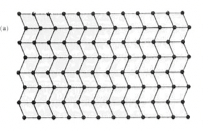
\includegraphics{images/img36.png}
\caption{Effetto della geminazione su un reticolo cristallino}
\labfig{img36}
\end{marginfigure}

Questi acciai hanno dunque molti vantaggi:
\begin{itemize}
    \item costano poco, in quanto contengono molto manganese, che è economico dato che è sempre presente nei minerali di ferro, e gli altri elementi non sono pregiati;
    \item si deformano in maniera elevatissima (fino al 50\%) grazie ai geminati
    \item hanno elevatissimi carichi di snervamento e di rottura, grazie ai meccanismi di incrudimento.
\end{itemize}

Gli acciai twip hanno però anche dei difetti:
\begin{itemize}
    \item le caratteristiche meccaniche crollano quando si effettuano processi di saldatura: si preferisce, quindi, usare adesivi o giunzioni rivettate;
    \item presentano il problema della corrosione, a causa dell’alto tenore di manganese;
    \item motivi economici, poiché fanno concorrenza ad altri acciai.
\end{itemize}

L'\textbf{acciaio TRIP}\index{acciaio TRIP} è un tipo di acciaio di plasticità indotta da trasformazione, è stato scoperto e nominato per la prima volta da VF Zackay, che ha utilizzato la trasformazione martensitica indotta da deformazione e la plasticità indotta in fase di austenite residua per migliorare la plasticità e la resistenza della lamiera di acciaio e migliorare la formabilità di lamiera di acciaio. Viene utilizzato principalmente per parti con struttura relativamente complessa, come la piastra di irrigidimento della colonna B e il raggio longitudinale anteriore dell'auto.

L'austenite residua è un residuo stabile della trasformazione dell'austenite. Quando la matrice viene trasformata in martensite, la parte residua può esistere solo come austenite a causa della limitazione dello spazio, che si chiama austenite residua. Nel processo di deformazione dell'acciaio TRIP, l'austenite residua viene trasformata in Martensite ad alto tenore di carbonio ad alta resistenza e, con l'espansione del volume, viene inibita l'instabilità della deformazione plastica e viene aumentato il campo di estensione uniforme, quindi la resistenza e la plasticità sono migliorati\footnote{Da: http://it.shew-esteelpipe.com/news/what-s-trip-steel-34103220.html consultato il 01/02/2021}.

\section{Superleghe}
Le superleghe sono leghe metalliche progettate per poter operare ad alte temperature, mantenendo delle buone proprietà meccaniche e senza ossidarsi, e sono per questo particolarmente ricercate per la costruzione delle turbine in campo aeronautico. \\
Le principali superleghe sono a base Nichel o a base Cobalto, con l'aggiunta di Cromo e Alluminio per aumentare la resistenza alla corrosione e all'ossidazione. Al contrario di quanto si suole fare per altri materiali metallici, nelle superleghe si cerca di ottenere cristalli i più grandi possibili, fino a ottenere una struttura monocristallina, per aumentare la resistenza al creep. Per incrementare questa caratteristica ulteriormente si può favorire la precipitazione di una seconda fase a bordo grano.
\begin{figure}[!hbt]
    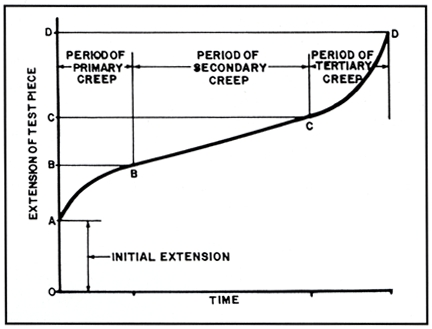
\includegraphics[width = 0.7\textwidth]{img40}
    \caption{Schema tempo deformazione per il fenomeno del creep}
    \labfig{img40}
\end{figure}
Il creep è infatti un fenomeno che si verifica alle alte temperature (una alta percentuale delle temperatura di fusione del materiale) consistente nello scorrimento reciproco dei grani, con conseguente deformazione anche a carico costante. La resistenza a questo fenomeno è quindi favorita dalla presenza di grani molto grandi e da precipitati che abbiano un'azione cementante.